\documentclass[aps,twocolumn,secnumarabic,balancelastpage,amsmath,amssymb,nofootinbib,floatfix]{revtex4-1}
\usepackage[a4paper, margin=1in]{geometry}
\usepackage{mathptmx} 
\usepackage{graphicx}
\usepackage{bm}
\usepackage[colorlinks=true]{hyperref} 
\usepackage[utf8]{inputenc} 
\usepackage[brazil]{babel}
\usepackage{url}
\usepackage{amsmath}
\usepackage{mathexam}
\usepackage{amsmath}
\usepackage{booktabs}


\begin{document}

    \title{Determinação do coeficiente de atrito estático usando o plano inclinado\LaTeX}
    \author{Enzo Totake}
    \email{enzo.totake@aluno.ufabc.edu.br}
    \author{Gustavo Jun Miyamoto Hassegawa}
    \email{gustavo.hassegawa@aluno.ufabc.edu.br}
    \author{Pedro Henrique Nakamura Otani}
    \email{pedro.otani@aluno.ufabc.edu.br}
    \author{Pedro Vitor Siqueira Guidil Pires}
    \email{pedro.guidil@aluno.ufabc.edu.br}
    \date{\today}
    \affiliation{Universidade Federal do ABC - UFABC}

    \begin{abstract}
        Este é um relatório acerca dos resultados obtidos em aula do experimento "Determinação do coeficiente de atrito estático usando o plano inclinado"
    \end{abstract}
    
    \maketitle
    
    \section{Introdução} 
        \subsection{Objetivos}
        \par O experimento teve como objetivo determinar o coeficiente de atrito estático \(\mu\) a partir do equilíbrio entre uma força no plano e a força de atrito estático num plano inclinado.
        
        \subsection{Contextualização e Importância}
        \par Compreender a força de atrito entre diferentes superfícies é fundamental para prever como materiais irão se comportar, tanto em movimento quanto em repouso. Em algumas situações, aumentar o atrito é desejável, como em freios, pneus, esportes, conexões mecânicas e pisos antiderrapantes, pois isso garante maior controle, segurança e estabilidade.
        \par Por outro lado, há casos em que a redução do atrito é vantajosa, como em motores, máquinas, sistemas de transmissão de energia, aeronaves, tubulações e na produção de eletrônicos. Nessas situações, diminuir o atrito melhora a eficiência, reduz o desgaste dos componentes e otimiza o desempenho dos sistemas.
        
    \section{Teoria}
        \subsection{Leis, princípios e teorias}

        \par O atrito é uma força que se opõe ao movimento entre duas superfícies em contato. Existem diferentes tipos de atrito, sendo o mais relevante para este experimento o atrito estático. O coeficiente de atrito (\(\mu\)) é uma medida adimensional que quantifica a intensidade do atrito entre duas superfícies.       
        \par O coeficiente de atrito estático (\(\mu_s\)) é determinado através da razão entre a força de atrito estático máxima e a força de reação normal que age sobre ele.
        \par A força de atrito estático atua para impedir que um objeto comece a se mover, até que atinja um valor máximo, dado pela fórmula(1).

        \begin{equation}
             F_{a_{\text{max}}} = \mu_s \cdot F_n
            \label{eq:Força de atrito estático}
        \end{equation}
        
        \subsection{Fórmulas}

        \par Neste experimento, será utilizado um plano inclinado, conforme ilustrado na Figura \ref{fig:aparato}. Esse arranjo permitirá medir a inclinação necessária para que um objeto comece a se mover.
        
        \begin{figure}[h]
            \centering
            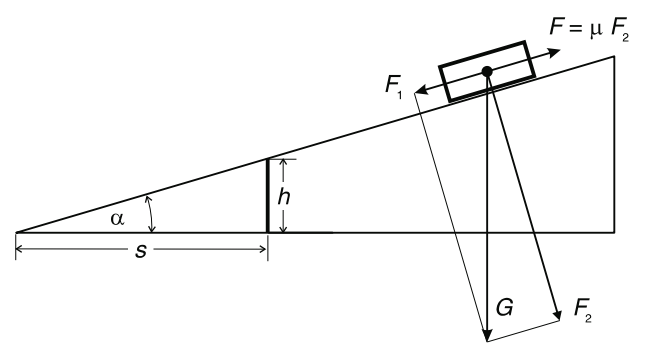
\includegraphics[width=.5\textwidth]{images/Labdefis.png}
            \caption{Representação do aparato experimental utilizado para a determinação do coeficiente de atrito. Imagem adaptada de Leybold.}
            \label{fig:aparato}
        \end{figure}

        \par Da imagem apresentada, seguem as seguintes equações:

        \par A força paralela ao plano é expressa pela equação:

        \begin{equation}
             F_1 = m \cdot \sin (\alpha)
            \label{eq:Força paralela ao plano}
        \end{equation}

        \par Enquanto a força perpendicular ao plano é dada por:
        
        \begin{equation}
             F_2 = m \cdot \cos (\alpha)
            \label{eq:Força perpendicular ao plano}
        \end{equation}

        \par A relação entre a altura (\(h\)) e a base (\(s\)) do triângulo formado pelo plano inclinado pode ser expressa pela tangente do ângulo (\(\alpha\)):
        
        \begin{equation}
             \tan(\alpha) =  \frac{h}{s}
            \label{eq:Relação tangente}
        \end{equation}

        \par A força de atrito estático também pode ser expressa como:
        
        \begin{equation}
            F_1 = F = \mu\ \cdot F_2 
            \label{eq:Força estática}
        \end{equation}

        \par Por fim, a relação do coeficiente de atrito em termos de altura e base é dada pela seguinte equação:
        
        \begin{equation}
            \mu\ = \frac{h}{s} 
            \label{eq:Relação do coeficiente de atrito}
        \end{equation}
           
    \section{Instrumentação e experimento}
        \subsection{Materiais utilizados}

        \subsection{Procedimentos}
    
    \section{Analise dos resultados}
        \subsection{Dados}
        
        \subsection{Análise e interpretação dos dados}
    
    \section{Conclusão}
    %Resumo dos principais achados do experimento
    %Se os objetivos foram alcançados e porquê
    
    \section{Referências}
    \begin{thebibliography}{9}
        \bibitem{leybold} Leybold Physics. Determining the coefficient of static friction using the inclined plane (P1.2.5.2). Disponível em: \url{https://www.leybold-shop.com/physics/physics-experiments/mechanics/forces/inclined-plane/determining-the-coefficient-of-static-friction-using-the-inclined-plane/vp1-2-5-2.html}
    \end{thebibliography}

\end{document}
